\chapter{Introduction}

%\chapter*{Introduction}
\label{intro}

% \par Introducere: obiectivele lucrarii si descrierea succinta a capitolelor, prezentarea temei, prezentarea contributiei proprii, respectiv a rezultatelor originale si mentionarea (daca este cazul) a sesiunii de comunicari unde a fost prezentata sau a revistei unde a fost publicata.
%THEME PRESENTATION
\section{Depression Statistics and Insights}
\label{sec:ch1sec1}

\par \quad Depression stands as a mental health affliction with profound impacts on both psychological and physical well-being. Characterized by a disinterest in routine activities, sleep disturbances, anhedonia, and in severe cases, suicidal ideation \cite{cui2015systematic}, it has become a problem across worldwide. Furthermore, individuals with major depressive disorder face a bigger risk of cardiovascular problems, not optimal treatment outcomes, and higher rates of morbidity and mortality \cite{seligman2015interface,luo2018effects}.

The World Health Organization (WHO) identifies depression as the primary contributor to global disability, affecting over 300 million individuals worldwide \cite{smith2014world}. Particularly alarming is the revelation that adolescents with severe depression are 30 times more prone to suicide \cite{stringaris2017depression}. 
Although we know depression is a big problem worldwide, we still don't fully understand what causes it. We know that cultural, psychological, and biological factors play a part, but we don't know exactly how they all fit together.\cite{gross2014silver,menard2016pathogenesis}.

The Global Burden of Disease (GBD) study \cite{liu2020changes} offers comprehensive insights into various mental problems across 195 countries, including depression. Divided into dysthymia and major depressive disorder categories, the GBD database from 1990 to 2017 furnishes valuable data for understanding depression's evolution globally. Major depressive disorder emerges as a predominant form of depression, posing a significant burden on global health, indicating it may become the leading cause of disability by 2030. Moreover, while dysthymia rates decreased in some regions, it remains a concern, particularly in the United States.

Identifying underlying causes and risk factors for depression, including genetic predisposition, demographic factors, unhealthy lifestyles, and diseases coming from it such as stroke, cancer, and AIDS, highlights the need for a change. Governments in countries with high depression rates are encouraged to prioritize research, promote healthy lifestyles, and ensure comprehensive care for individuals with predisposing conditions. However, the study acknowledges limitations in data analysis, advocating for future research of regional risk factors and guide tailored policy interventions for effective depression control globally. This can be seen in Figure \ref{FigGloablDepression} \cite{liu2020changes}, which evaluated the worldwide burden of depression using the estimated annual percentage change (EAPC) and age-standardized incidence rate (ASR).

\begin{figure}[htbp]
	\centering
		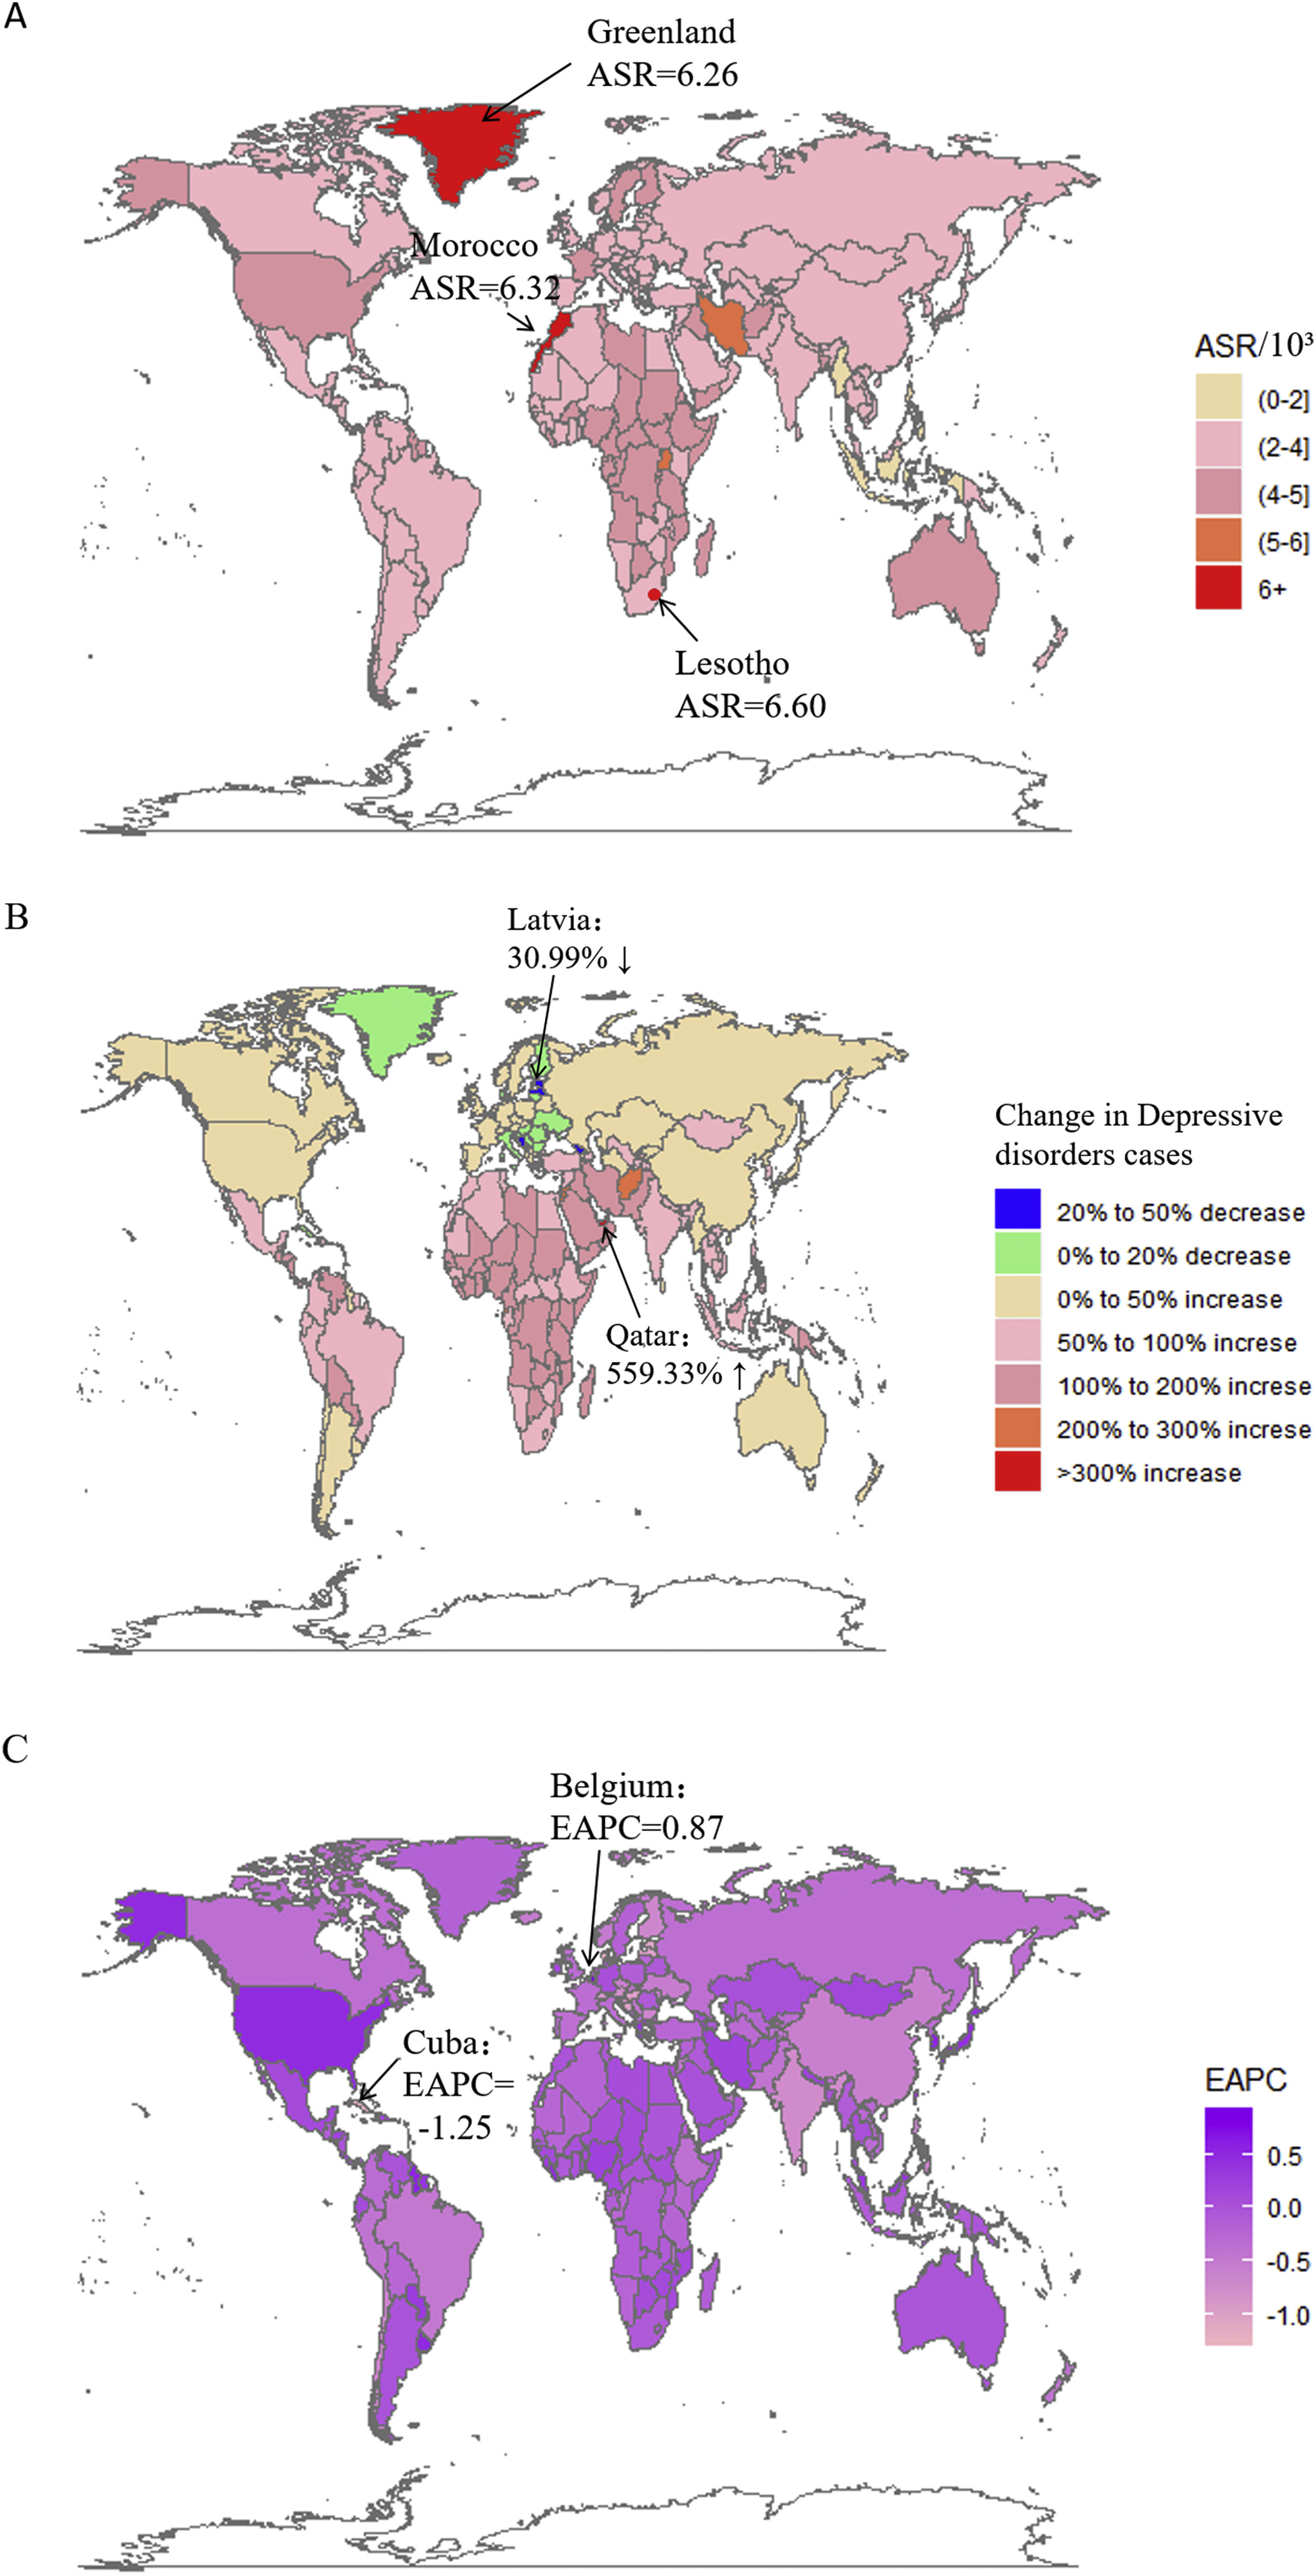
\includegraphics[scale=0.65]{./figures/depression-map-Liu-et-al-2020.jpg}
	\caption{Global depression statistics comparison between 1990 and 2017 \cite{liu2020changes}}
	\label{FigGloablDepression}
\end{figure}

\section{Objective}
\label{sec:ch1sec2}

\quad The objective of our scientific study is to leverage machine learning techniques to develop a tool for identifying depression through textual analysis. By harnessing the power of natural language processing (NLP) and artificial intelligence (AI), we aim to create a fast and reliable tool capable of detecting signs of depression in text-based communications.

We aim to achieve two things. Firstly, we seek to provide an accessible application of identifying individuals who may be experiencing symptoms of depression. By analyzing the language used in written communications, such as social media posts, emails, or chat messages, our tool aims to offer an initial assessment of an individual's mental well-being. This approach can facilitate early intervention and support, potentially preventing more severe depressive symptoms and their associated consequences.

Secondly, we aim to evaluate the performance of our machine learning model in a cross-linguistic context. To achieve this, we will translate our dataset from English to Romanian and assess the performance of the model on both language versions. This comparative analysis will enable us to tell if of our tool is accurate across different languages and cultural contexts.

With this study we hope to contribute to the advancement of computational techniques for mental health assessment and intervention. Our aim is to provide clinicians, researchers, and individuals themselves with a valuable resource for early detection and prevention of depression, ultimately encouraging improved mental well-being and quality of life.